\section{Control de Formaciones con Consenso en Sistemas No Holonómicos }
\subsection{Estructura Virtual con Generador de Trayectorias}

\begin{figure*}[h]
    \centering
    \begin{tikzpicture}[
      font=\fontfamily{ptm}\selectfont\scriptsize,
      >={Stealth[length=2mm]},
      block/.style={draw, minimum width=1.3cm, minimum height=1.3cm, align=center, inner sep=2pt},
    ]
      \node[block] (VS) {Estructura\\Virtual};
      \node[block, right=1.1cm of VS] (C)  {Consenso};
      \node[block, right=1.1cm of C]  (CL) {Ley de\\Control};
      \node[block, right=1.1cm of CL] (F)  {PVA};

      \node[align=center, above=0.7cm of C] (NB) {Vecindad};
      \node[align=center, above=0.7cm of F] (LI) {LiDAR};

      \draw[->] (VS) -- node[above]{$x_v$} node[below]{$[x,y]$} (C);
      \draw[->] (C)  -- node[above]{$z$} node[below]{$[a,\alpha]$} (CL);
      \draw[->] (CL) -- node[above]{$u_{ref}$} node[below]{$[v,\omega]$} (F);
      \draw[->] (NB) -- (C);
      \draw[->] (LI) -- (F);

      \coordinate (uEnd) at ($(F.east)+(0.8,0)$);
      \draw[->] (F.east) -- node[above]{$u^*$} node[below]{$[v,\omega]$} (uEnd);
    \end{tikzpicture}
    \caption{Estrategia de control de formación}
    \label{fig:flujo_control}
\end{figure*}
\section{Control de Formaciones con Consenso en Sistemas No Holonómicos }
\subsection{Estructura Virtual con Generador de Trayectorias}

\begin{center}
\ifshow
    \animategraphics[autoplay,loop,height=4.4cm]{10}{Pics/vs_frames/vs-}{0}{743}
\else
    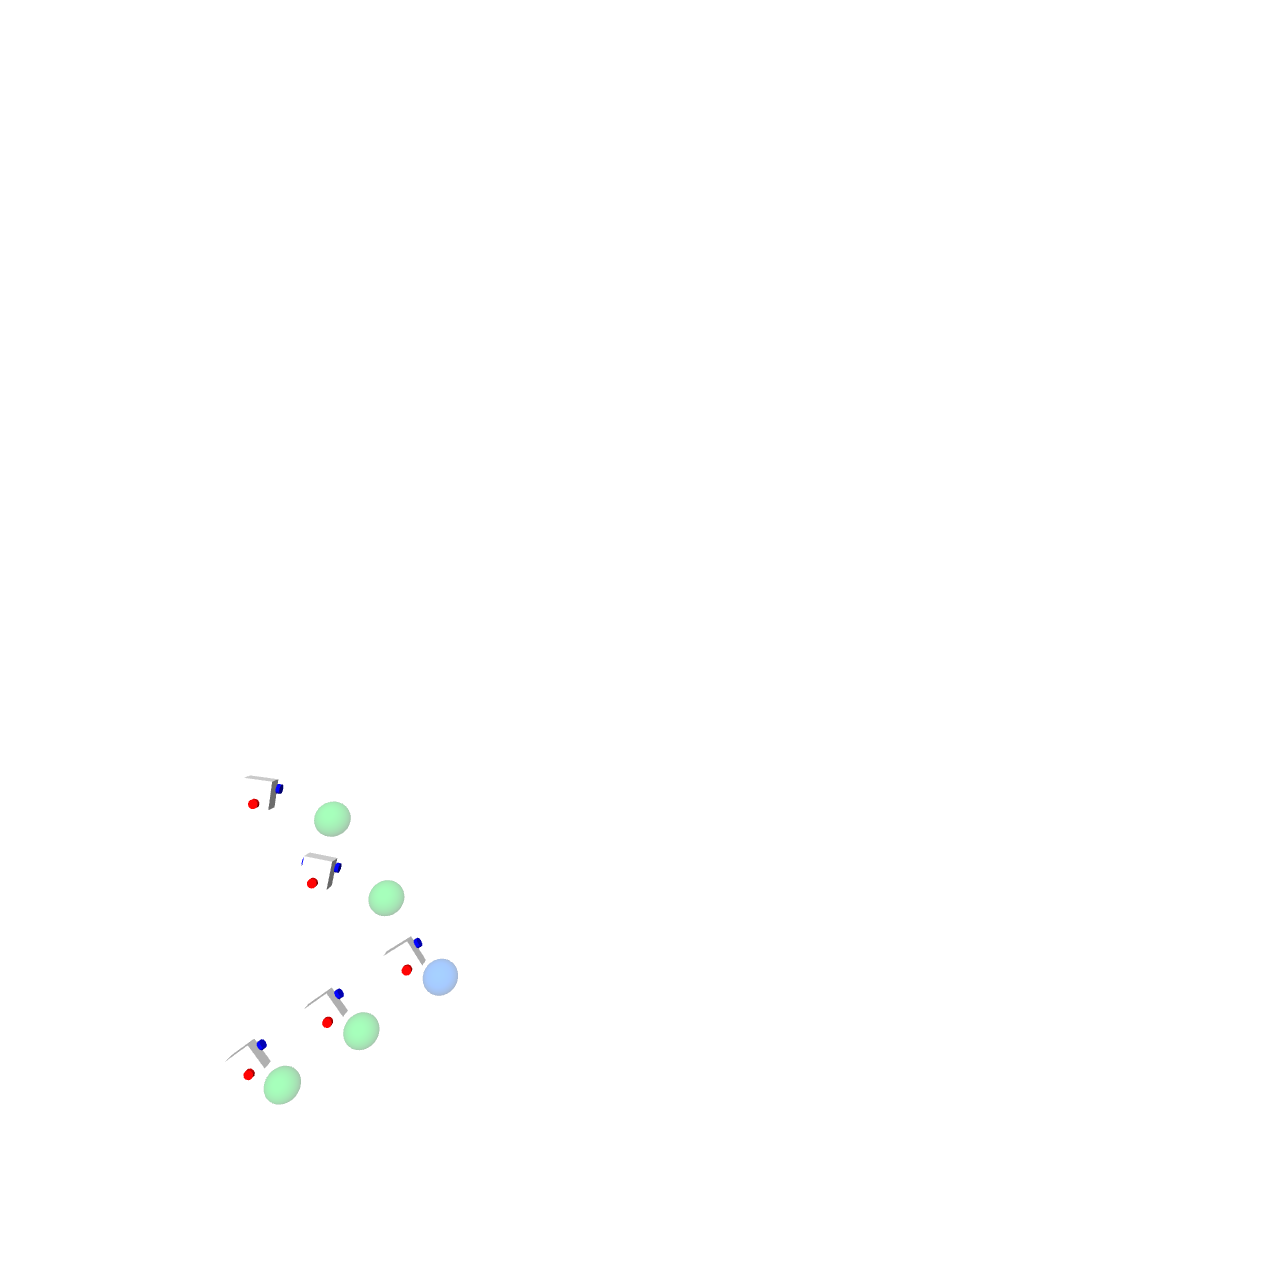
\includegraphics[height=4.4cm]{Pics/vs_frames/vs-370.png}
\fi
\end{center}
\begin{center}
\footnotesize Simulación en Gazebo de la estructura virtual siguiendo su trayectoria
\end{center}

\section{Estructura Virtual con Obstáculos}
\subsection{Evasión de Mínimos Locales sin Atrapamiento}
